%!TEX root = ../master.tex
\chapter{Design}\label{ch:design}
\todo{This part needs rework. Write after chapter is done.}
This chapter will cover the design iterations and the decisions that were made. 


\section{Peripheral devices}
The user has to be able to affect a pre-existing audio file by interacting with a physical interface. The system with apply an affect which can be modified through a physical scalar which changes the variable range of the power of the effect from 0\% to 100\%, or in digits 0 to 1. For this interface these different variations of a physical scalar has been considered: 

\begin{itemize}
\item Pedal
\item Joystick
\item Variable resistor
\item Bend sensor
\end{itemize}

\begin{figure}[!h] 
\centering
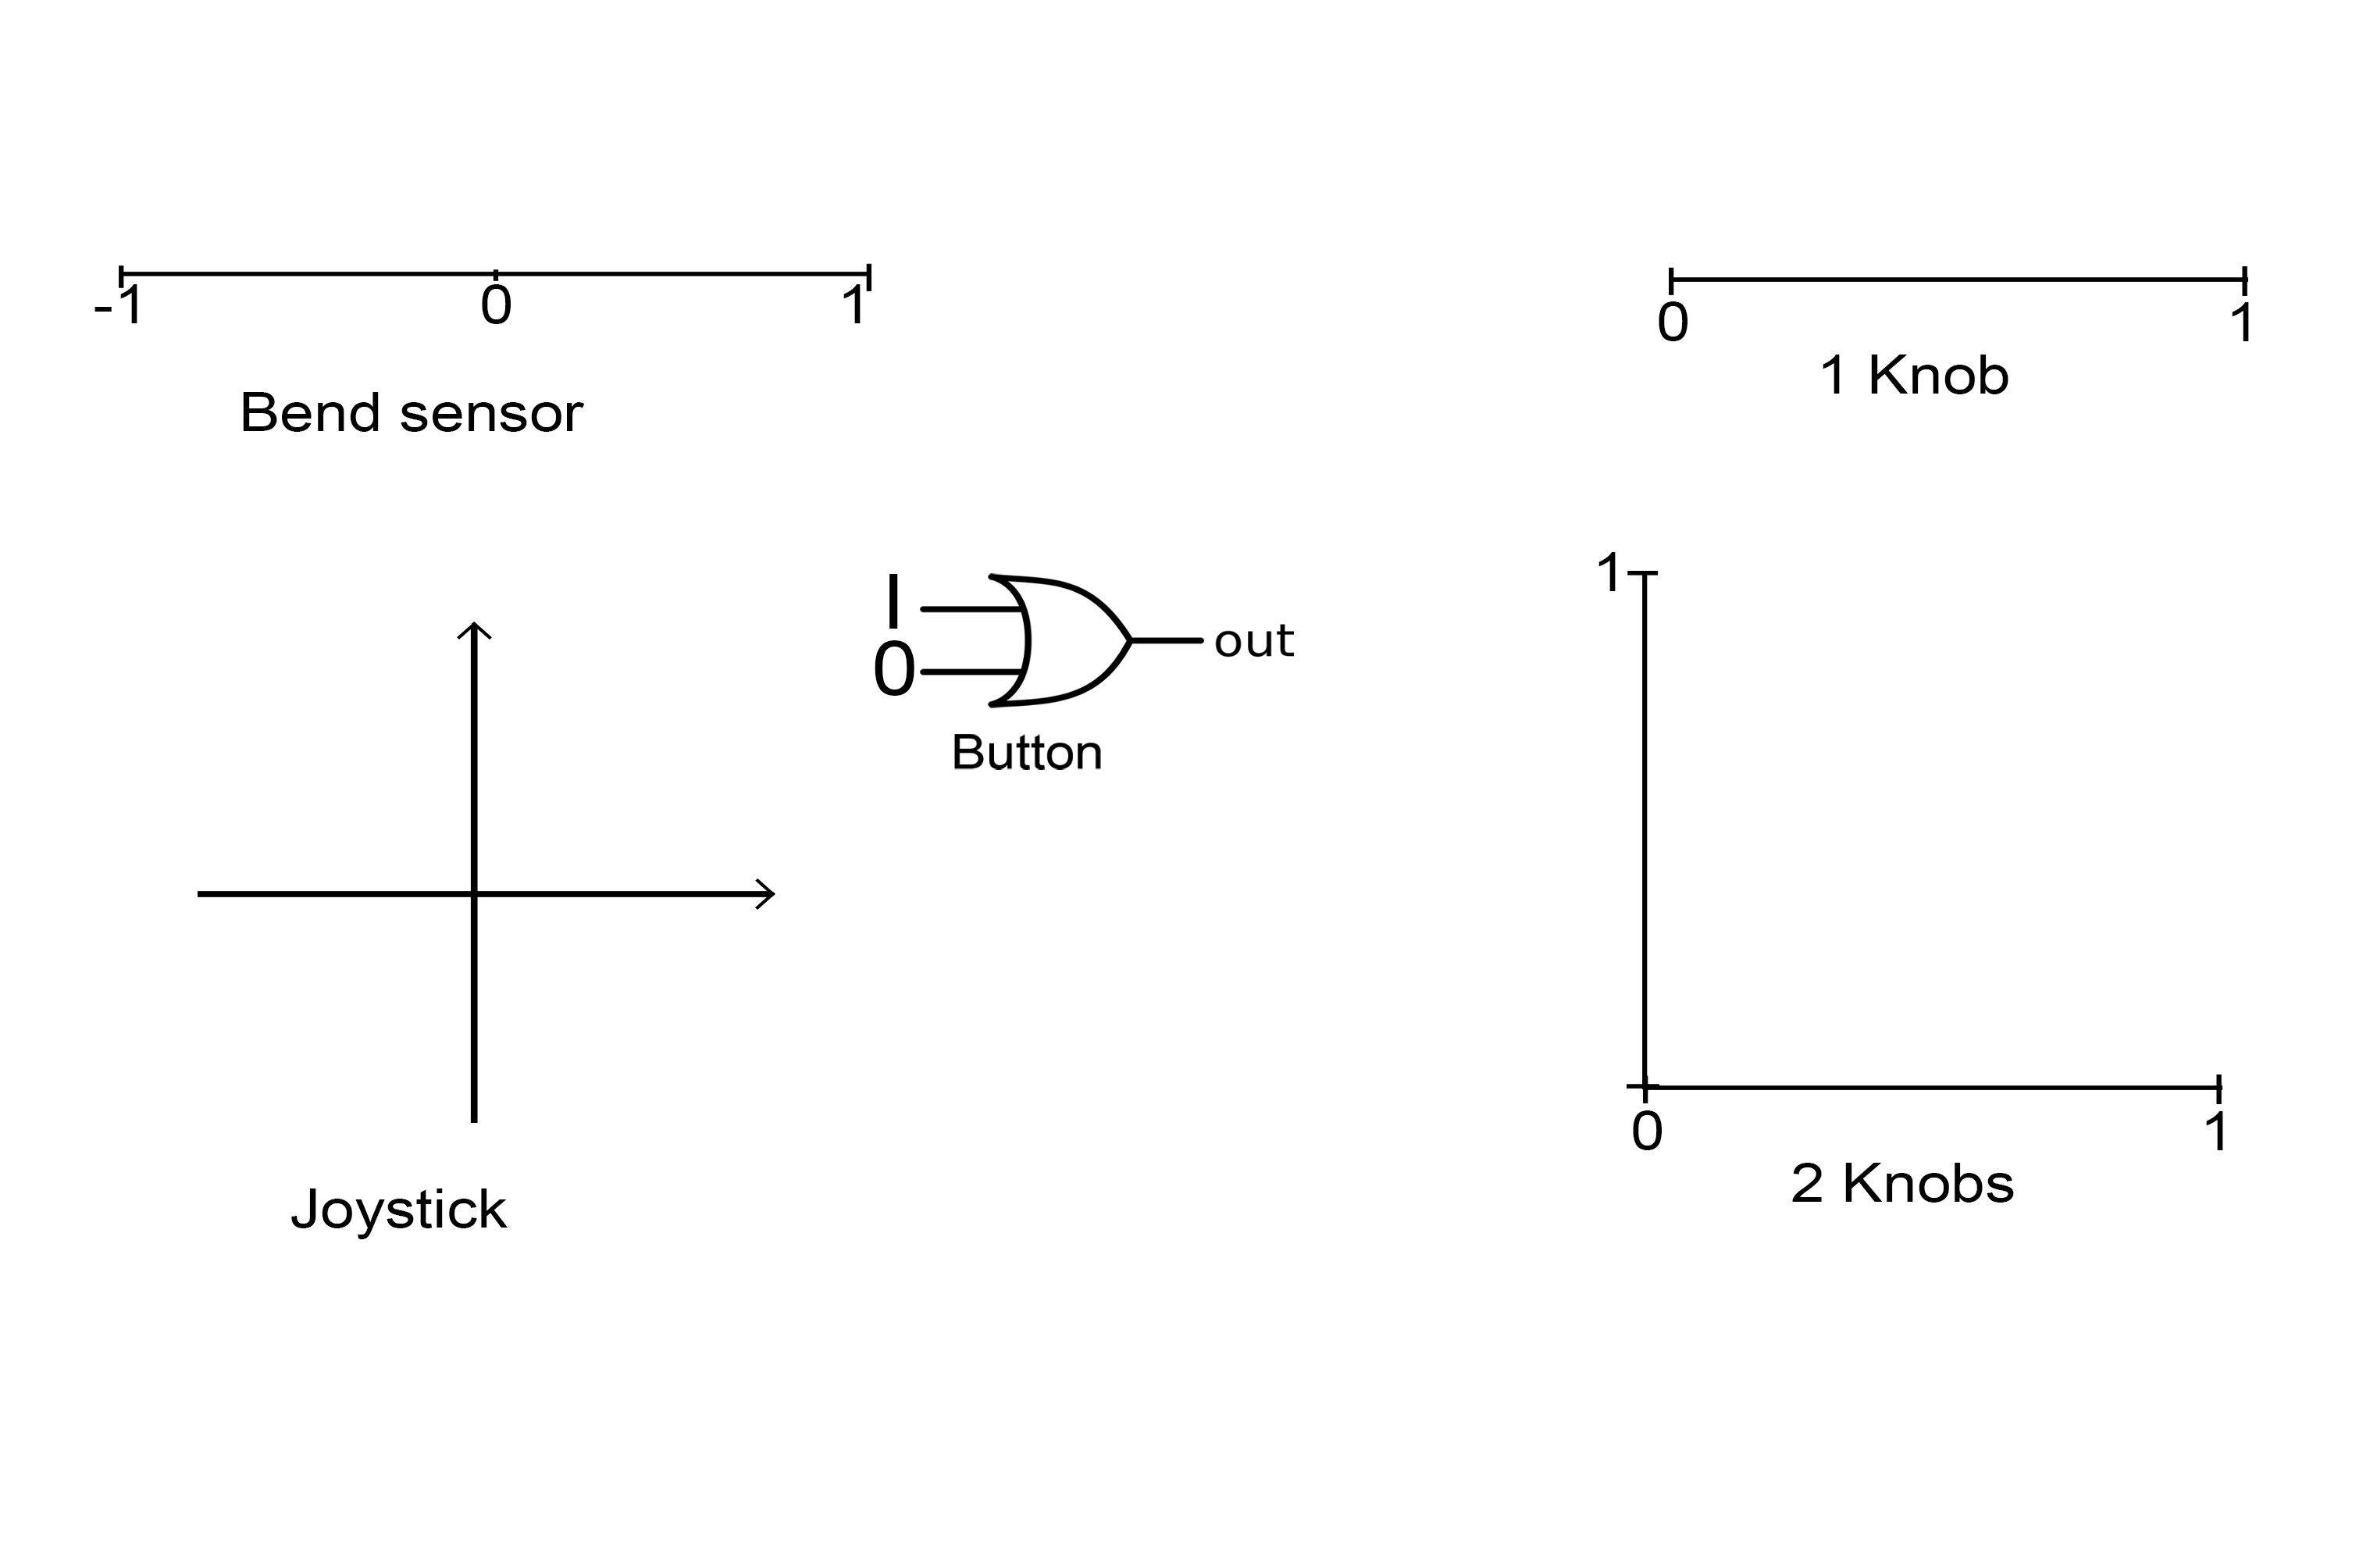
\includegraphics[width=1\textwidth]{Axis}
\caption{\label{fig:axis}}
\end{figure}


\todo{talk about what is the preference of different interfaces for the user (after test)}

Each of these peripheral devices makes the user interact with the prototype differently and changes the function of each device.

Figure \ref{fig:axis} shows the scales of which the different devices operate on, and how many different axis they are able to manipulate and to what length.
 
The joystick work by incorporating a variable on each axis, such that when the joystick is moved it alters the variables on the axis. 

There are multiple variable resistors to choose from. One of them being a knob the user can turn, which scales from 0 to 1 as well as a bend sensor that scales from negative 1 to positive 1. When the user alters the resistance in the system, the Arduino registers the change and send back a signal to the software in order to change the effect.

The way that these devices would be used, are as variable controller for the effect itself. Depending on what device is chosen, the integration for the user will be different. This will be tested in the iterations of the prototype and discussed further to make sure that the interface is user-friendly and easy to understand. 

\todo{expand upon the advantages and disadvantages of the different categories of devices}
